\begin{figure}[H]
\centering
\subfigure{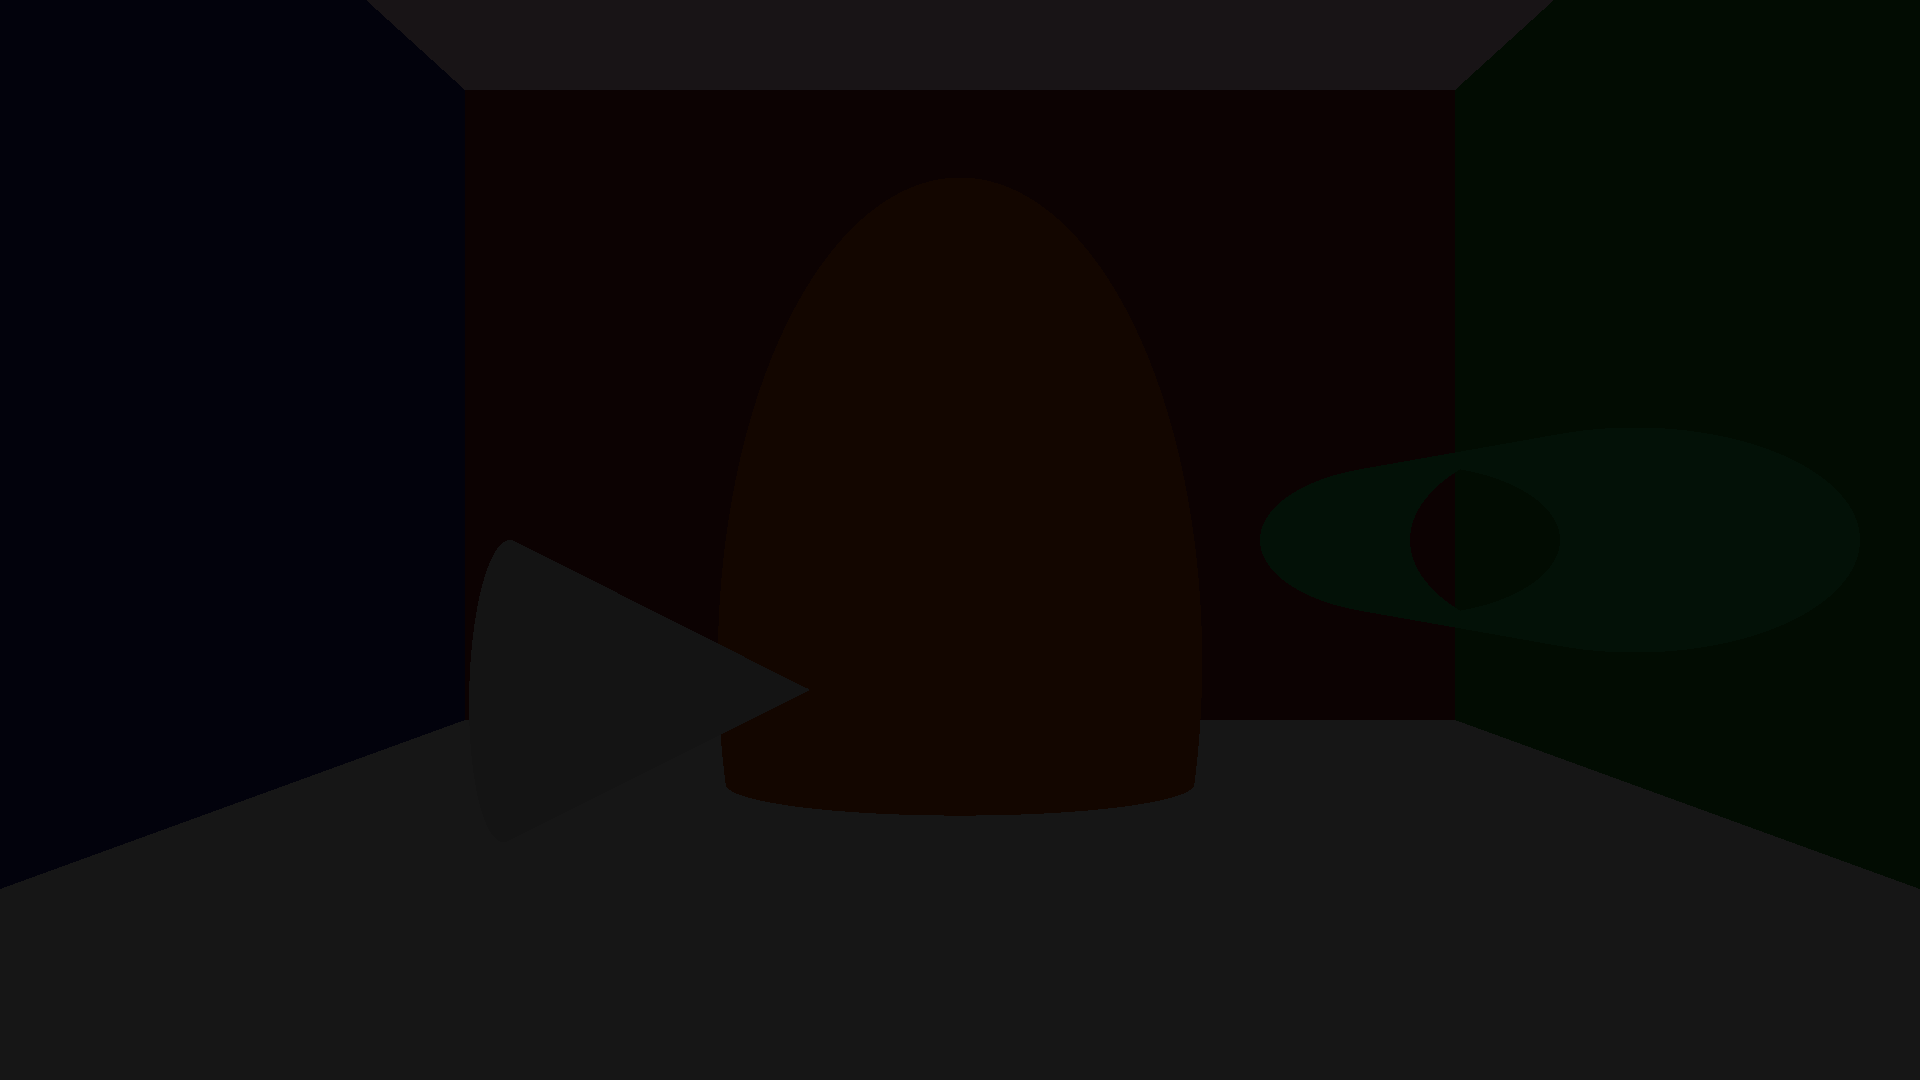
\includegraphics[width=0.45\textwidth]{chapters/ch3/img/complexity/0.png}}
\subfigure{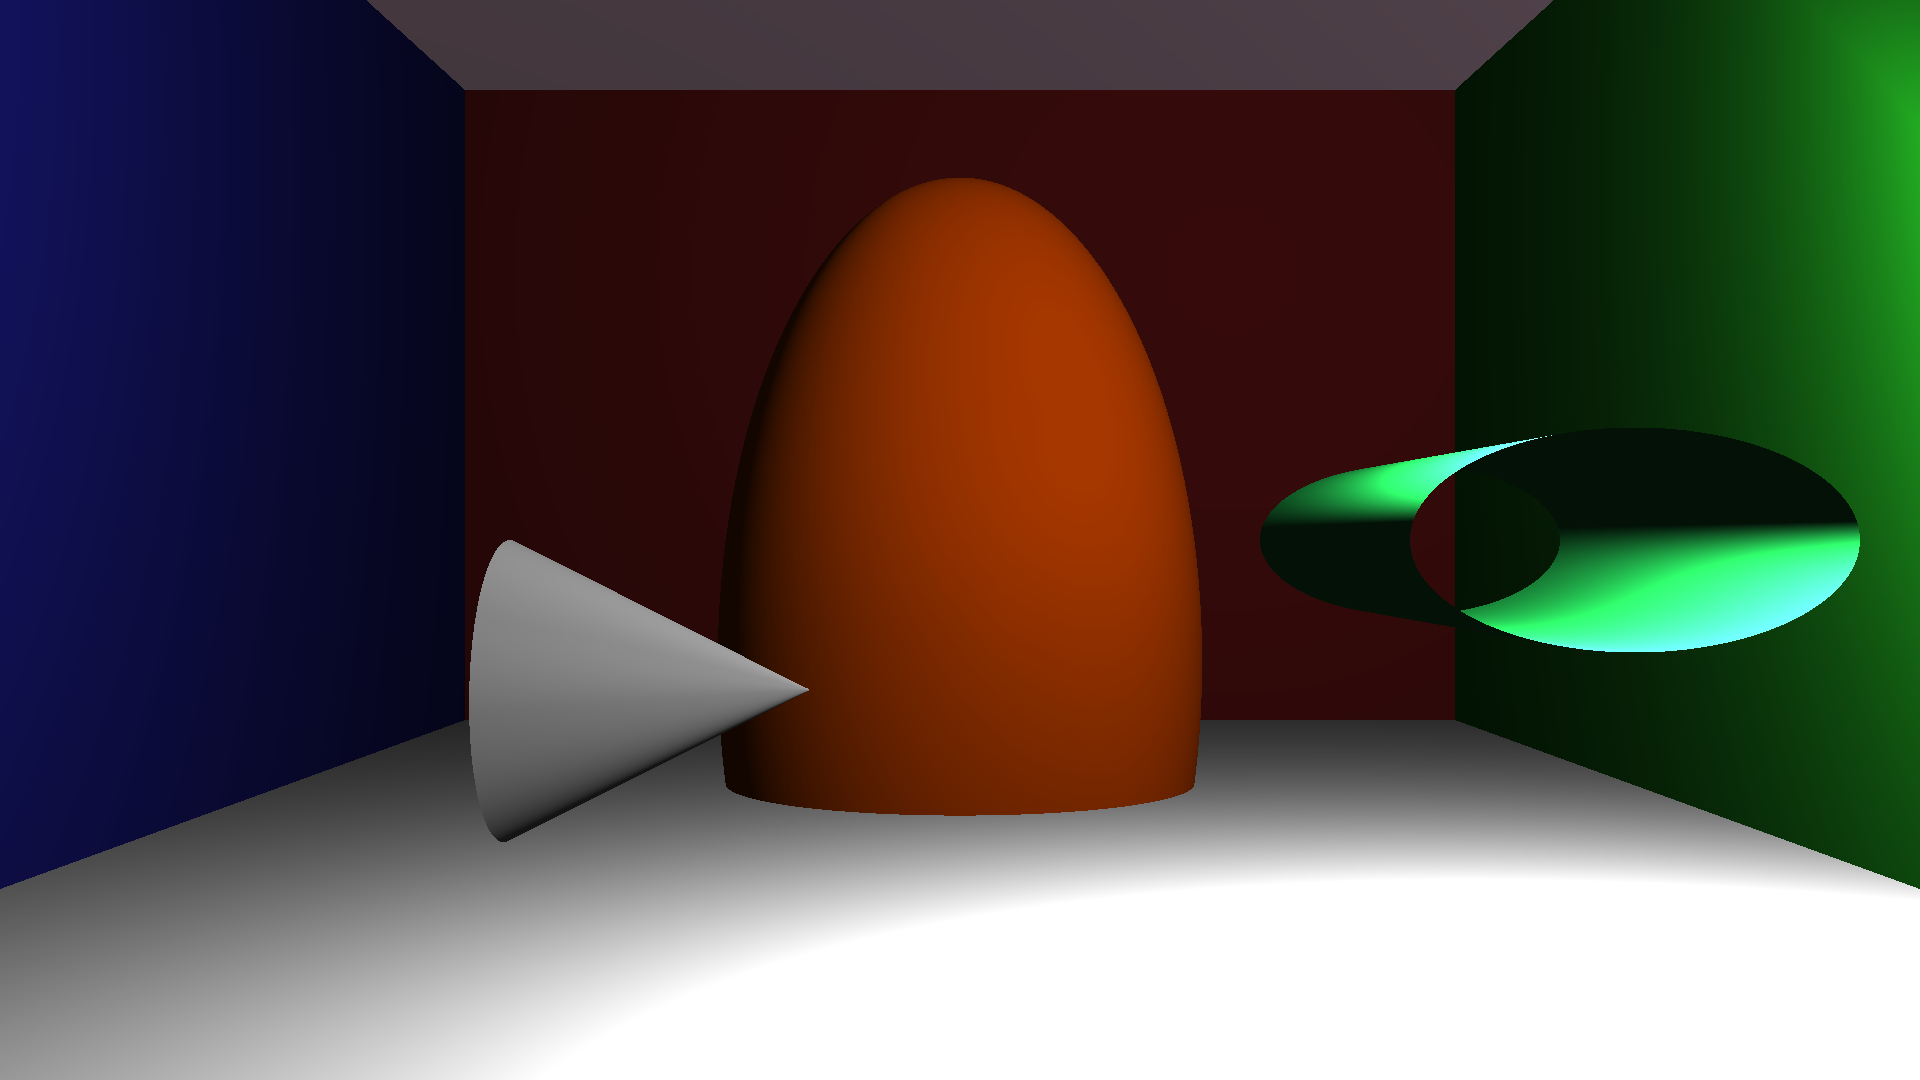
\includegraphics[width=0.45\textwidth]{chapters/ch3/img/complexity/1.png}}

\subfigure{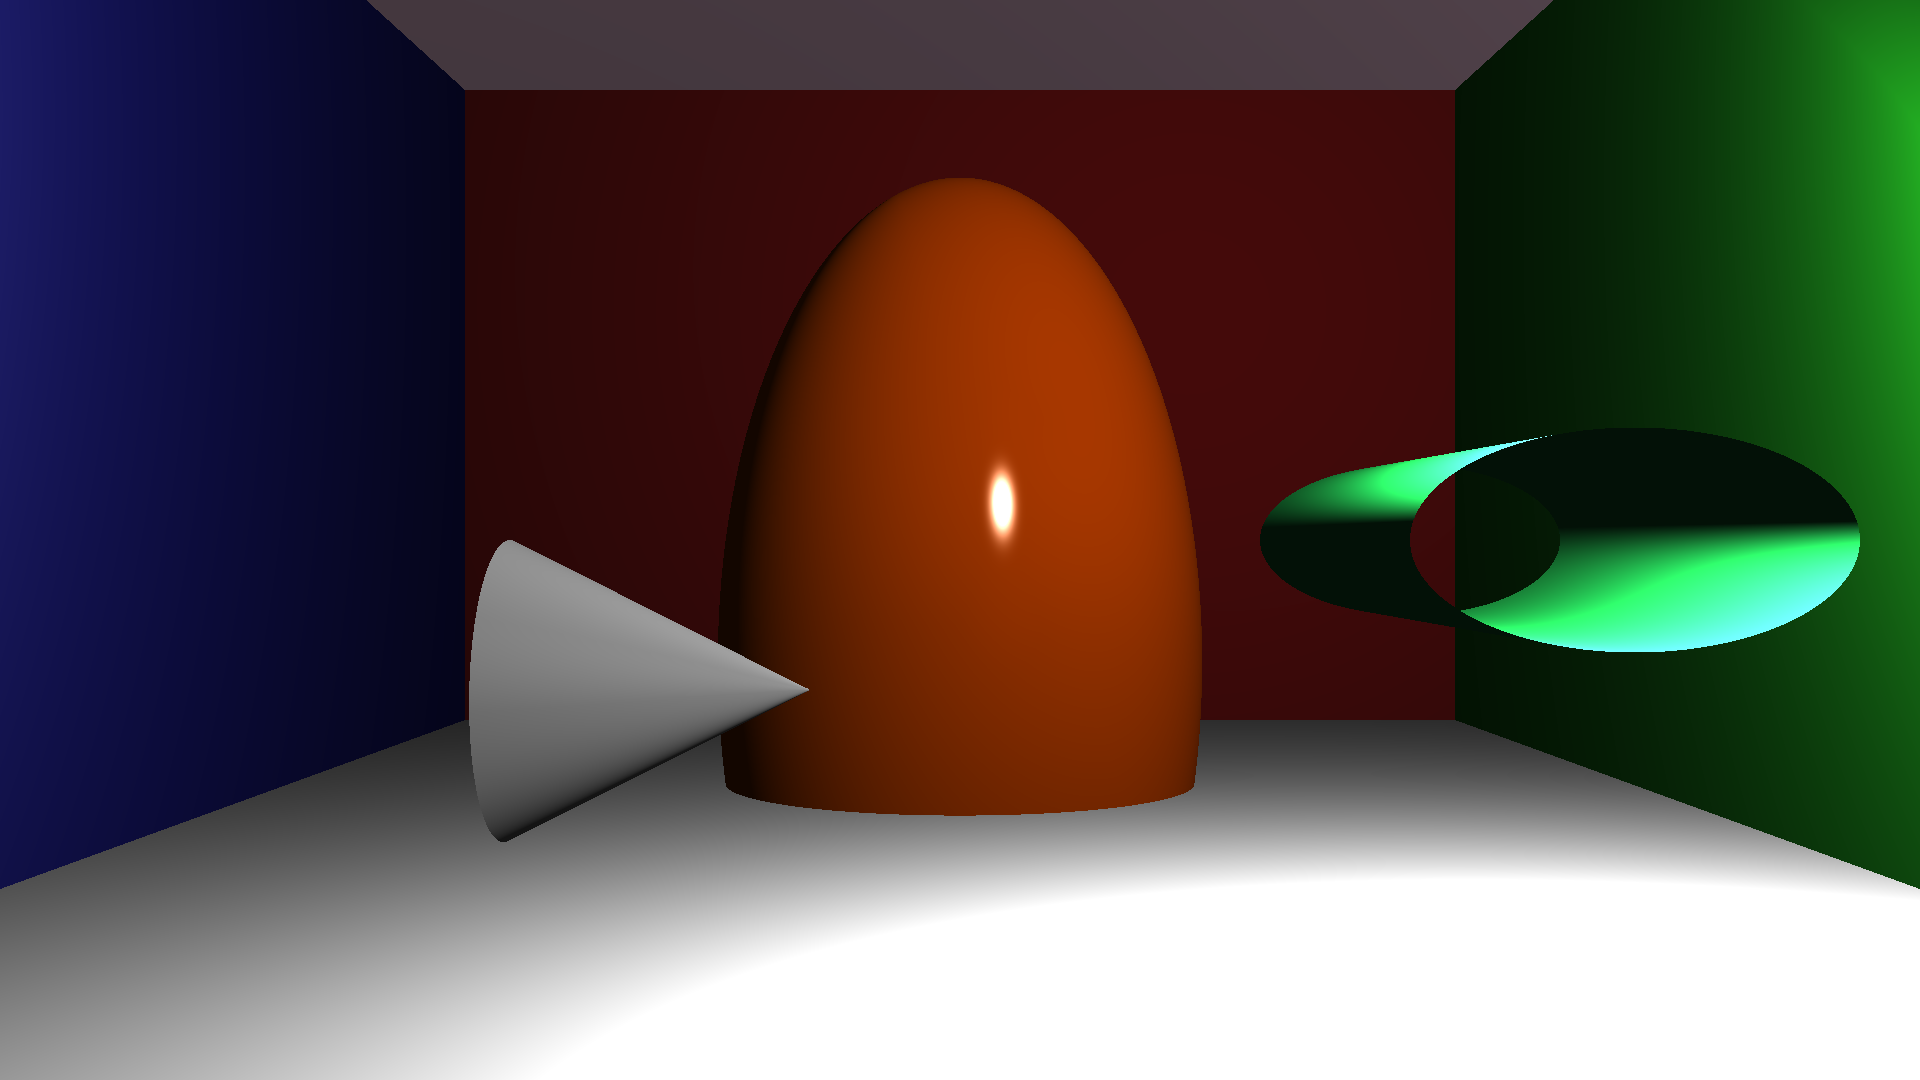
\includegraphics[width=0.45\textwidth]{chapters/ch3/img/complexity/2.png}}
\subfigure{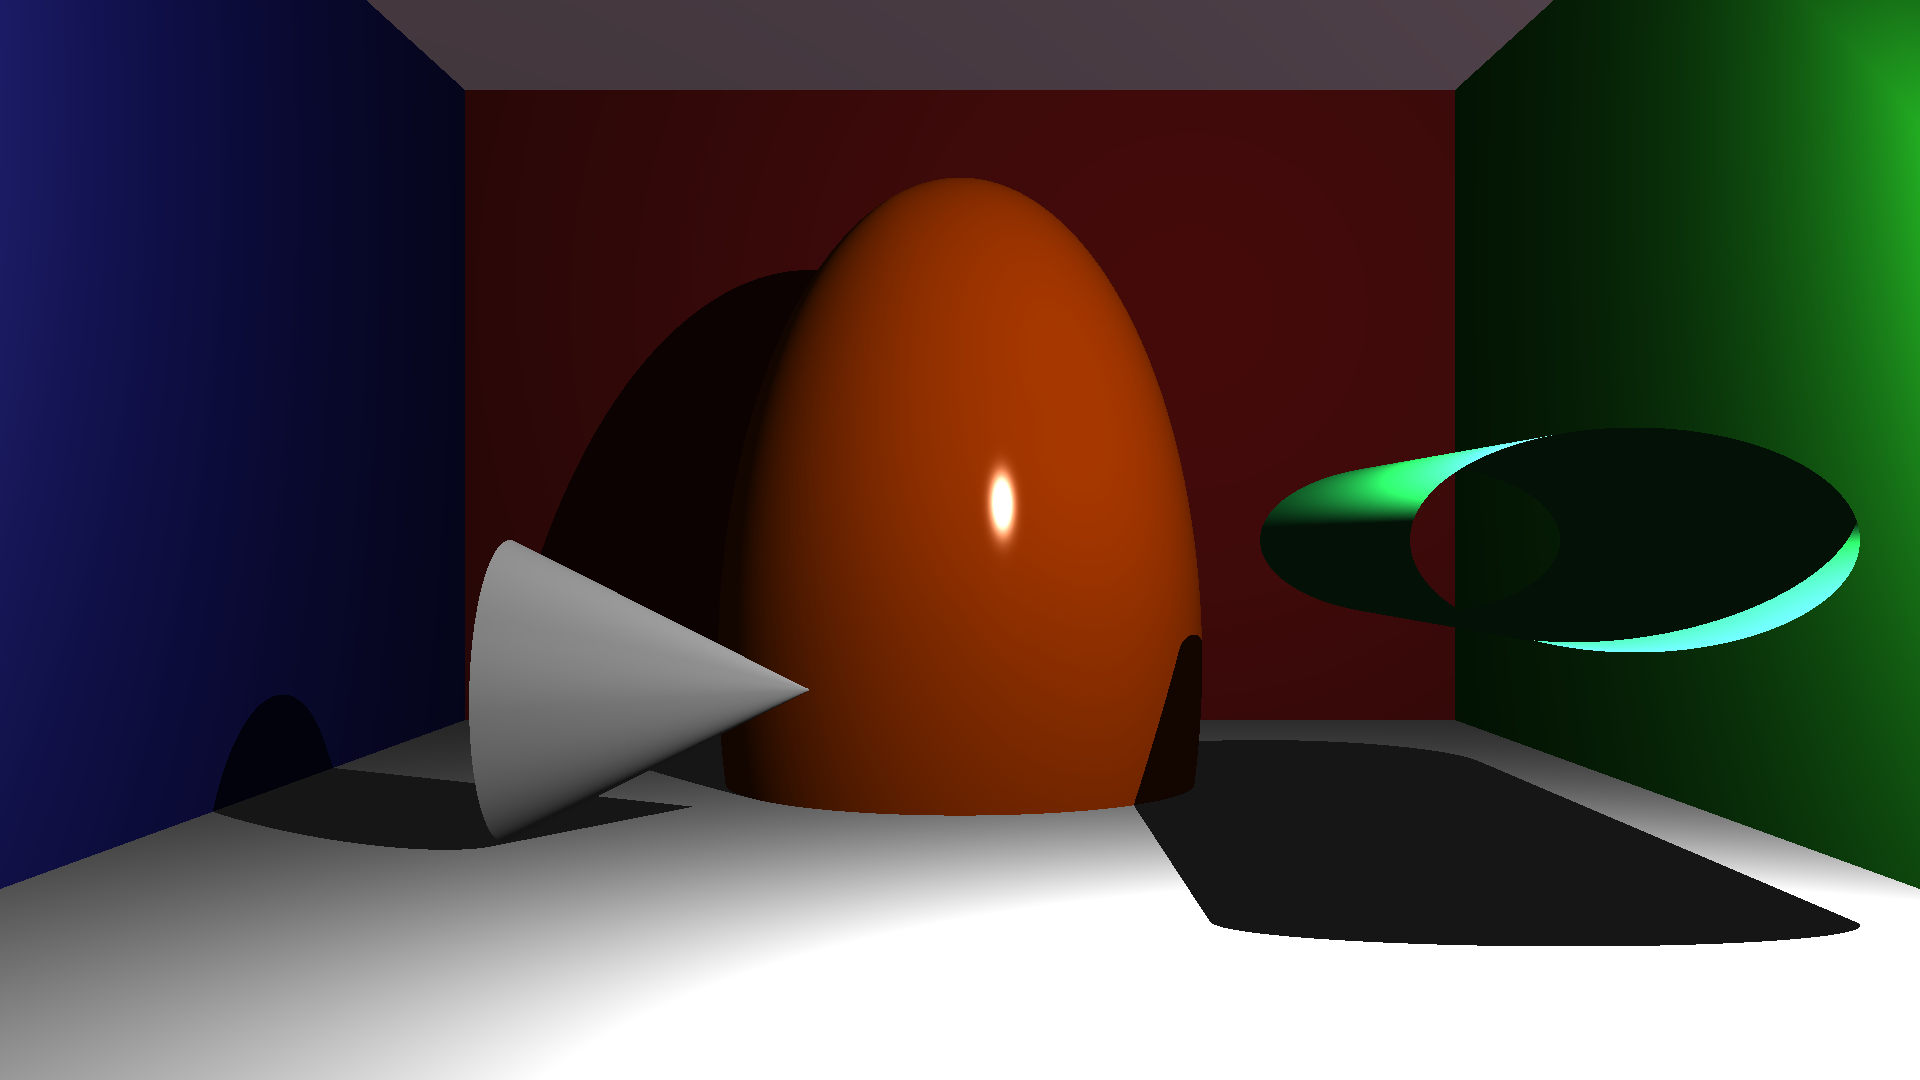
\includegraphics[width=0.45\textwidth]{chapters/ch3/img/complexity/3.png}}

\subfigure{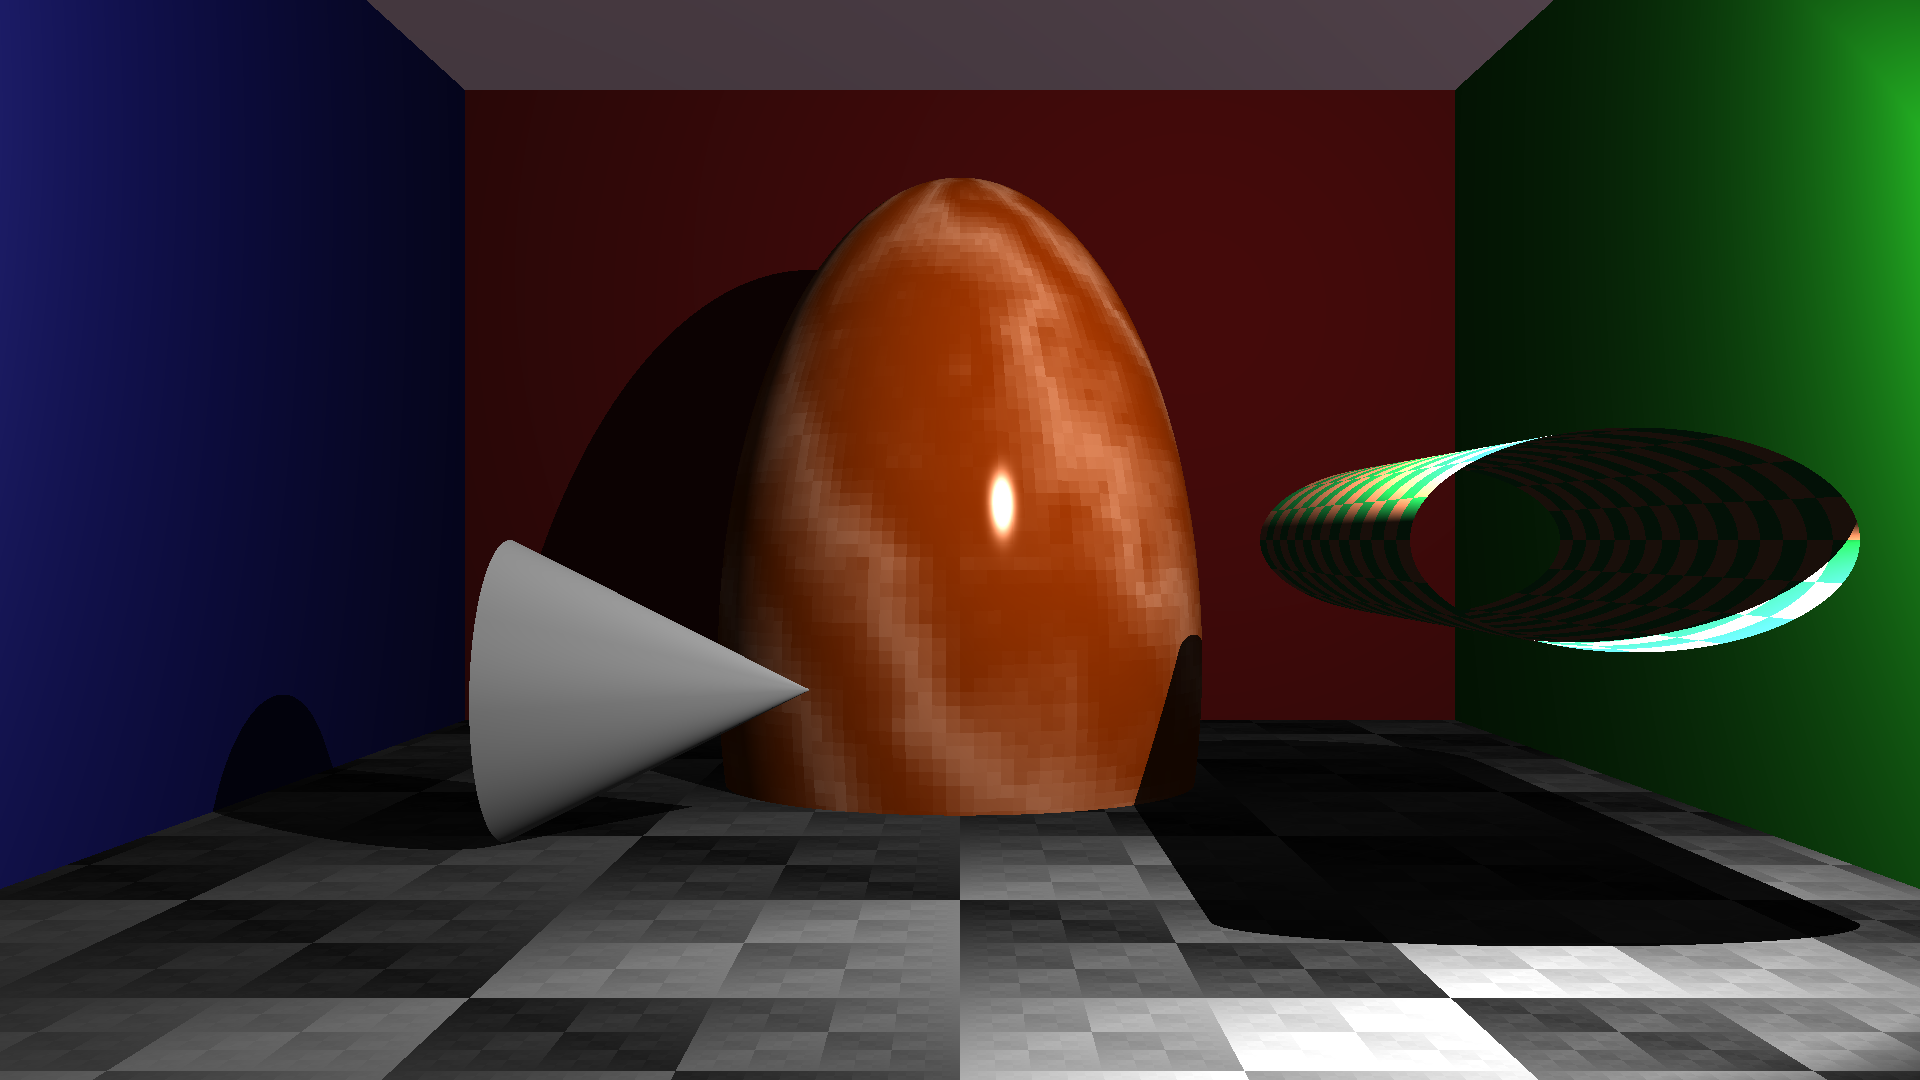
\includegraphics[width=0.45\textwidth]{chapters/ch3/img/complexity/4.png}}
\subfigure{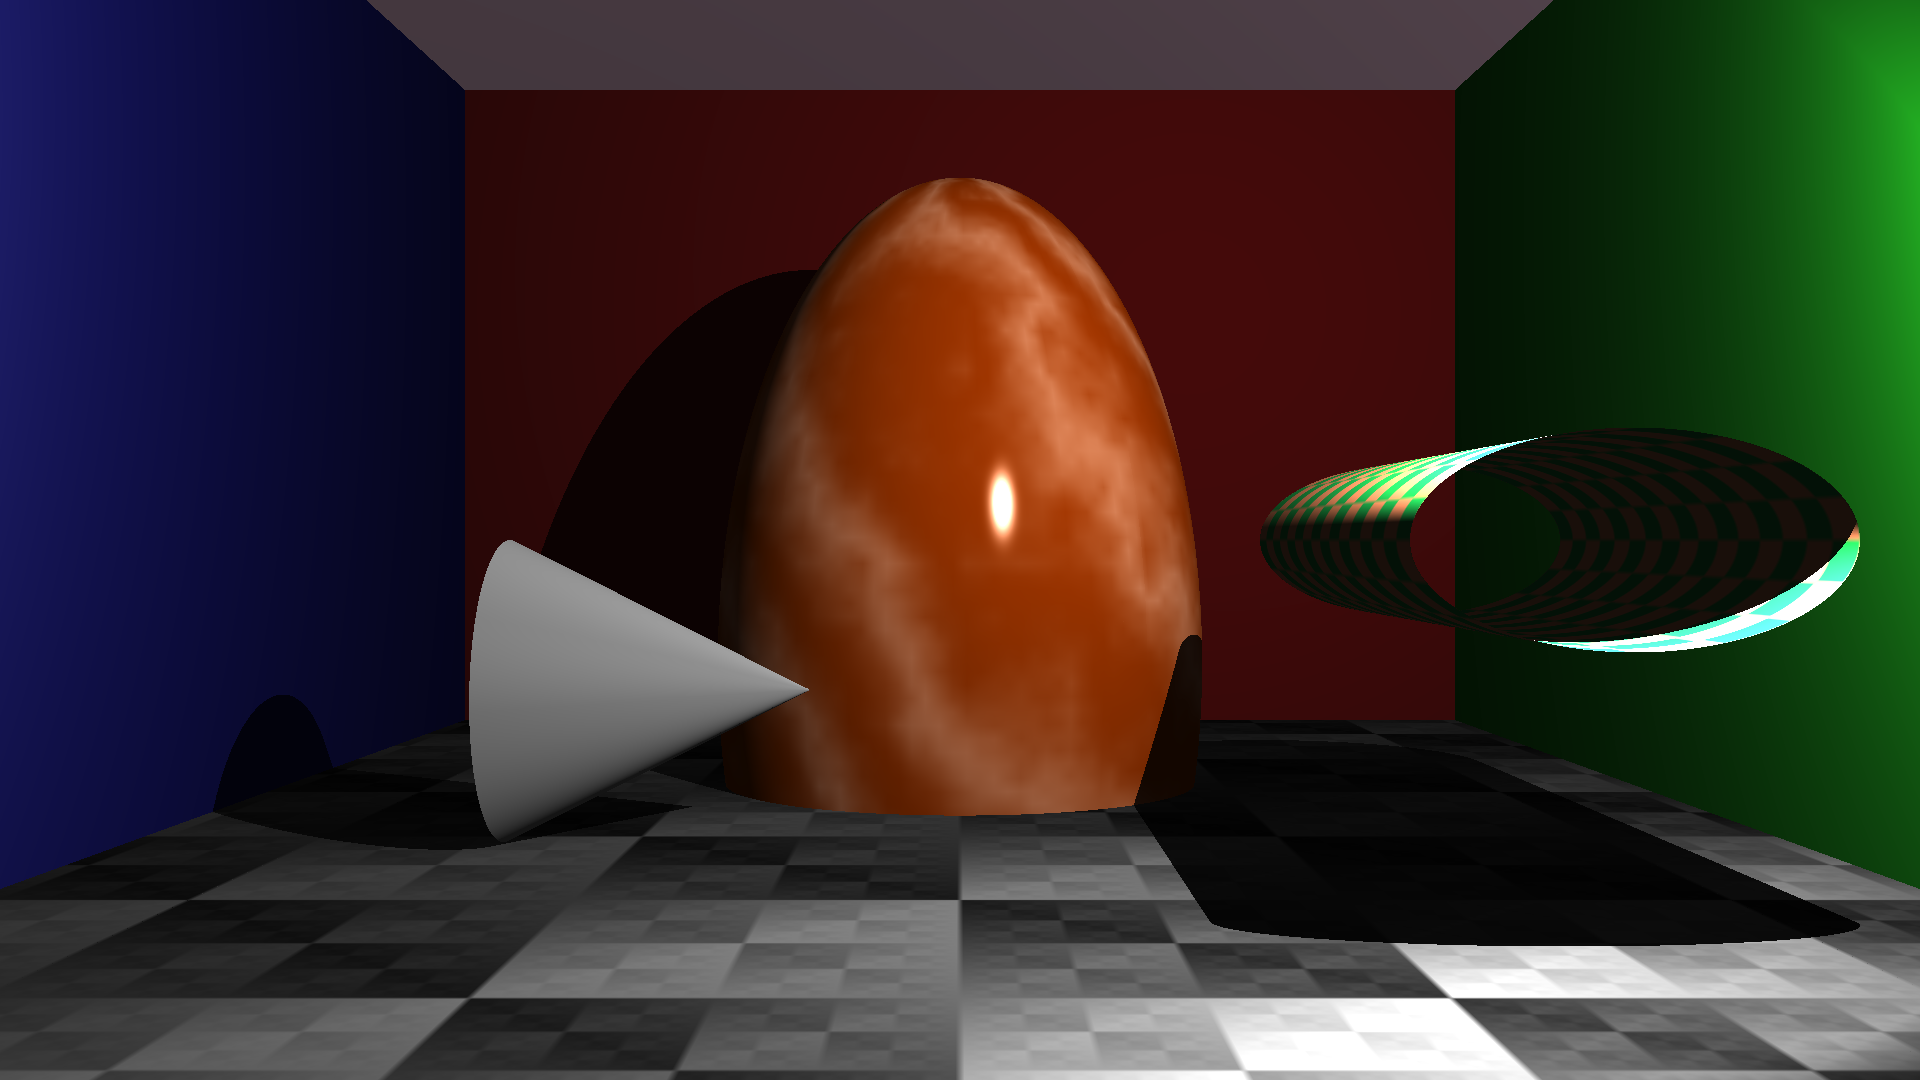
\includegraphics[width=0.45\textwidth]{chapters/ch3/img/complexity/5.png}}

\subfigure{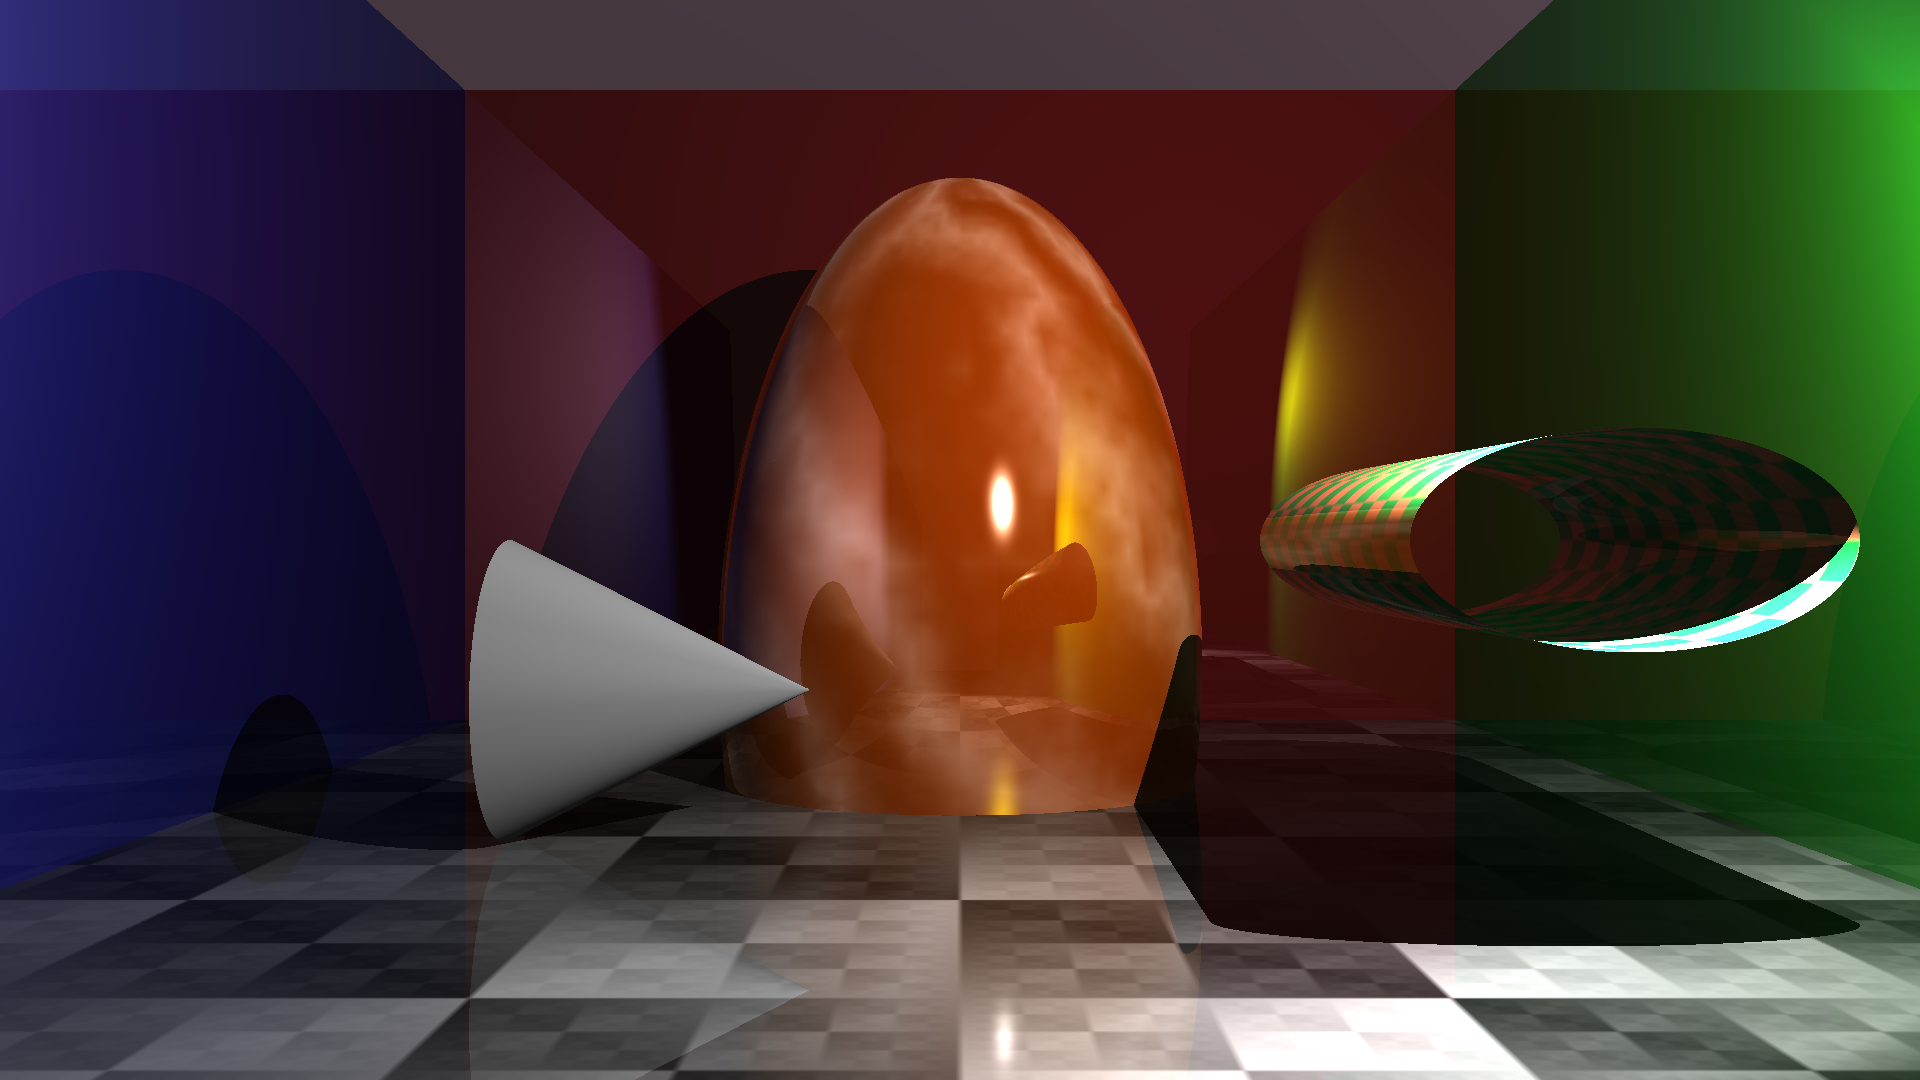
\includegraphics[width=0.45\textwidth]{chapters/ch3/img/complexity/6.png}}
\subfigure{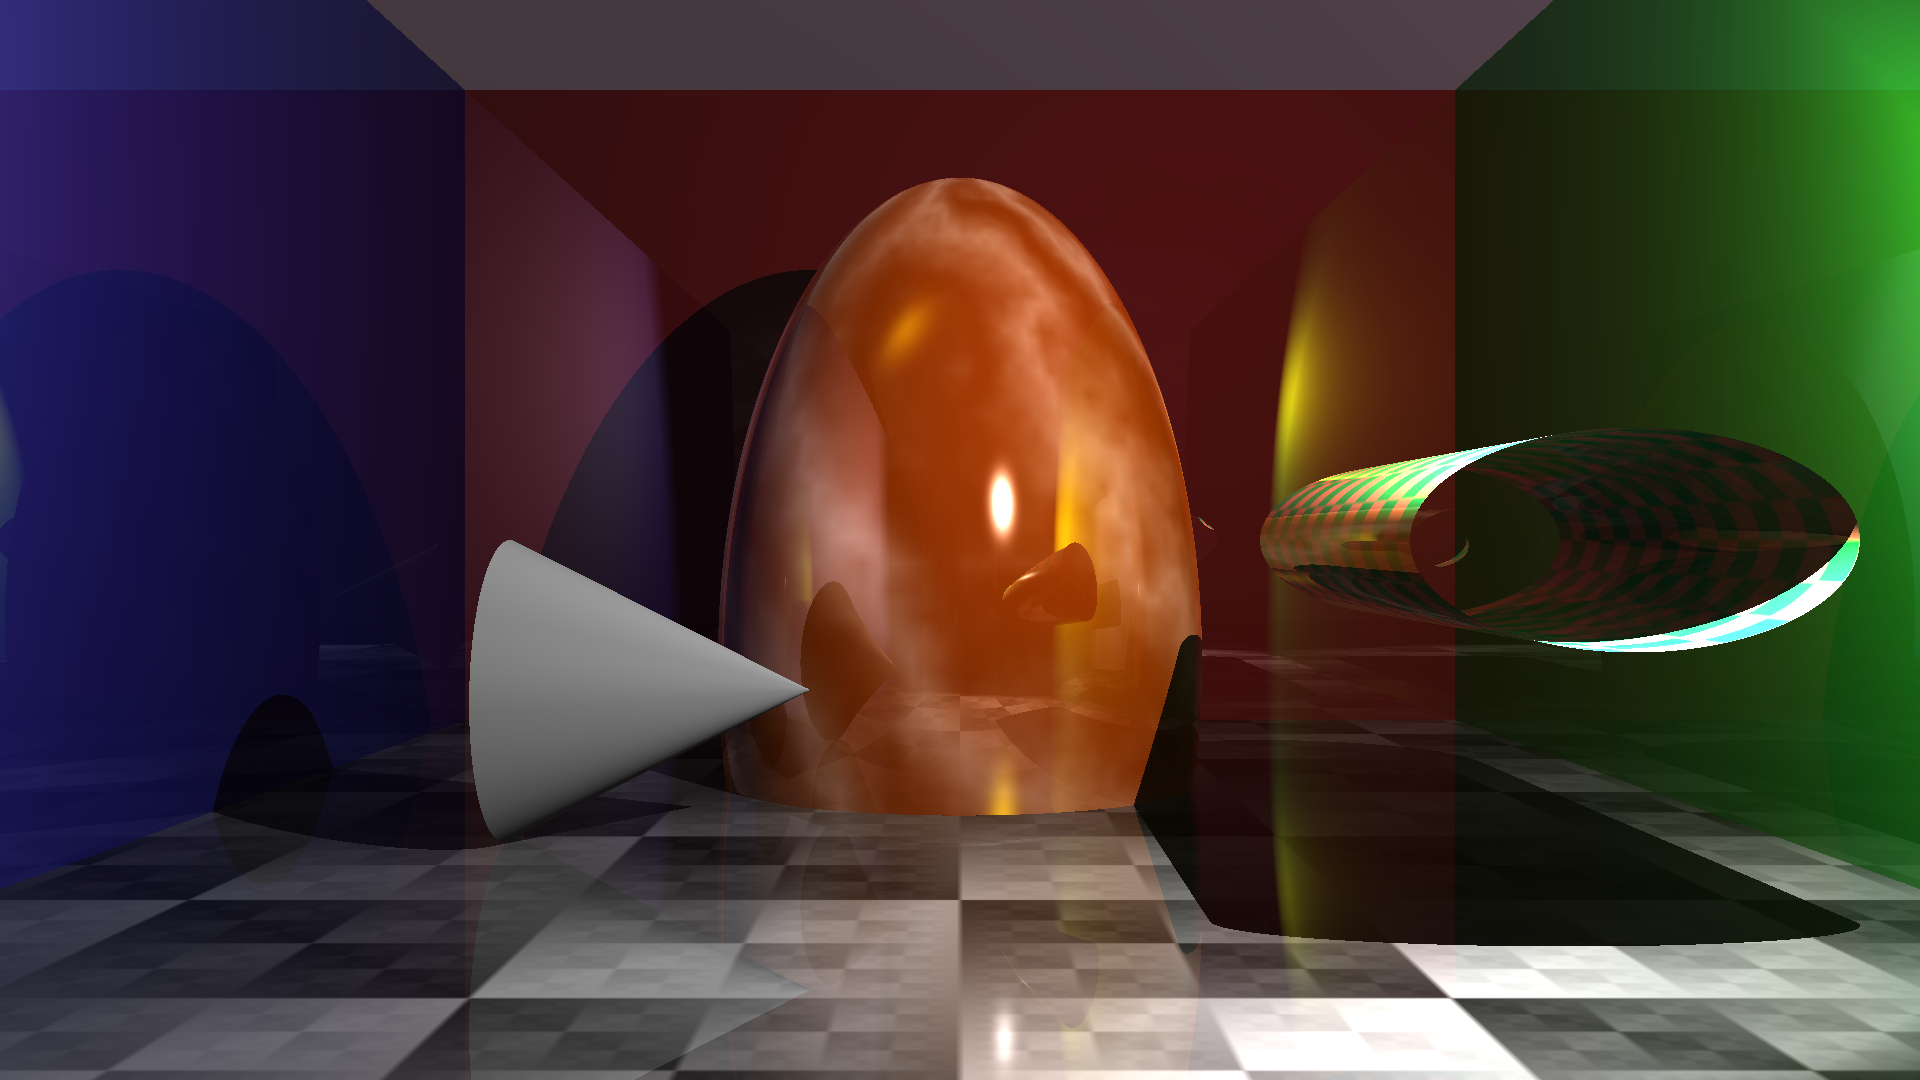
\includegraphics[width=0.45\textwidth]{chapters/ch3/img/complexity/7.png}}

\subfigure{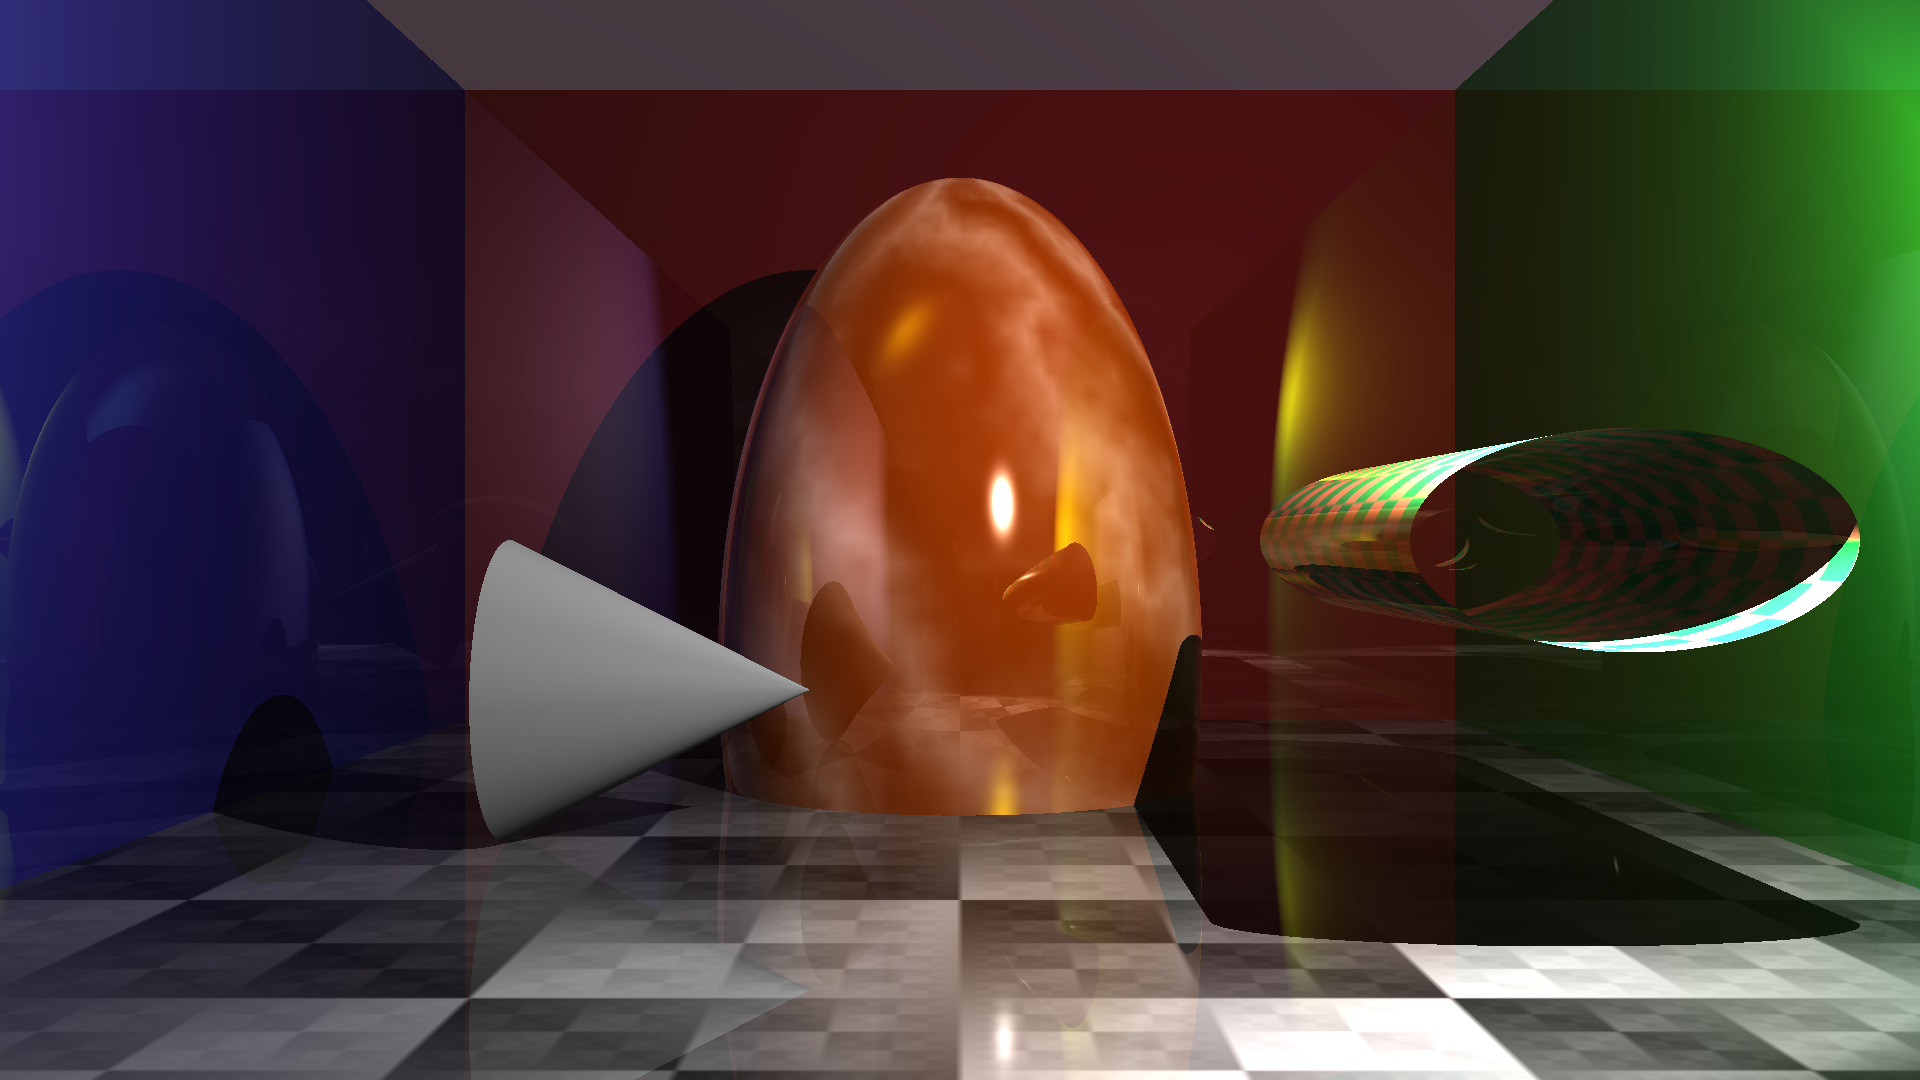
\includegraphics[width=0.45\textwidth]{chapters/ch3/img/complexity/8.png}}
\subfigure{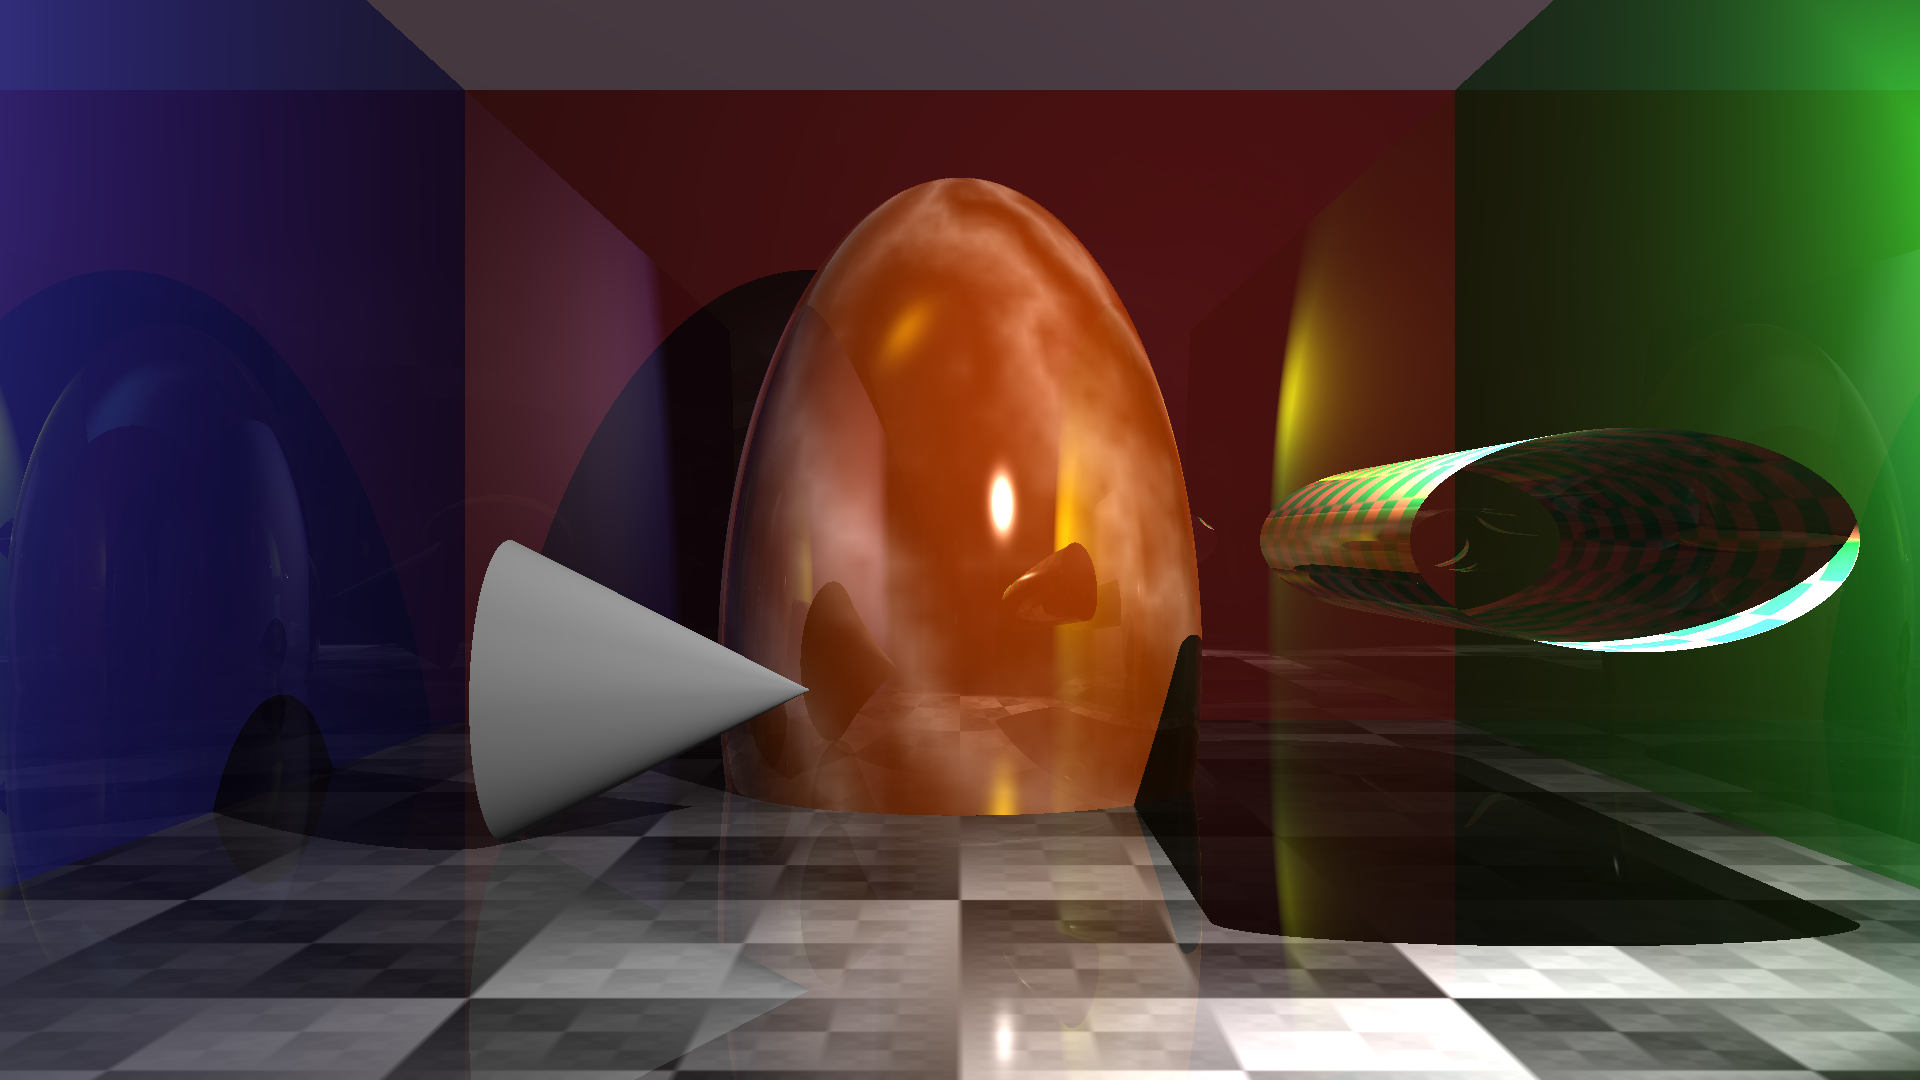
\includegraphics[width=0.45\textwidth]{chapters/ch3/img/complexity/9.png}}


\caption[Wpływ konfiguracji na poziom komplikacji generowanego obrazu]{Wpływ konfiguracji na poziom komplikacji generowanego obrazu. Umożliwienie generowania cieni, a następnie włączenie obliczeń związanych z tworzeniem odbić na~powierzchniach najbardziej wpływają na realizm przedstawionej sceny.}
\label{ch3:img:complexity}
\end{figure}